\section{Questão 158 - Unidades de medida, proporcionalidade, Regra de 3, Geometria}

Comum em lançamentos de empreendimentos imobiliários, as maquetes de condomínios funcionam como uma ótima ferramenta de marketing para as construtoras, pois, além de encantar clientes, auxiliam de maneira significativa os corretores na negociação e venda de imóveis.

Um condomínio está sendo lançado em um novo bairro de uma cidade. Na maquete projetada pela construtora, em escala de 1 : 200, existe um reservatório de água com capacidade de $ 45 cm^3 $.

Quando todas as famílias estiverem residindo no condomínio, a estimativa é que, por dia, sejam consumidos 30 000 litros de água. 

Em uma eventual falta de água, o reservatório cheio será suficiente para abastecer o condomínio por quantos dias?

(A)  30

(B)  15

(C)  12

(D)  6

(E)  3


\textbf{Resolução}

\noindent \resizebox{.5\textwidth}{!}{
    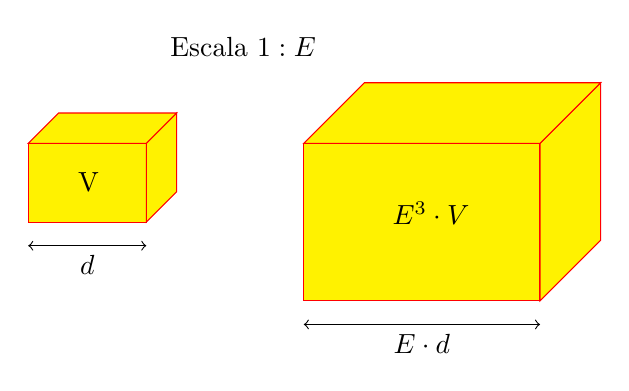
\begin{tikzpicture}
        
        \pgfmathsetmacro{\cubex}{1.5};
        \pgfmathsetmacro{\cubey}{1};
        \pgfmathsetmacro{\cubez}{1};
        
        \pgfmathsetmacro{\cubeX}{3};
        \pgfmathsetmacro{\cubeY}{2};
        \pgfmathsetmacro{\cubeZ}{2};
        
        
        \draw [red,fill=yellow] (0,0,0) -- ++(-\cubex,0,0) -- ++(0,-\cubey,0) -- ++(\cubex,0,0) -- cycle;
        \draw [red,fill=yellow] (0,0,0) -- ++(0,0,-\cubez) -- ++(0,-\cubey,0) -- ++(0,0,\cubez) -- cycle;
        \draw [red,fill=yellow] (0,0,0) -- ++(-\cubex,0,0) -- ++(0,0,-\cubez) -- ++(\cubex,0,0) -- cycle;
        
        \draw[red,fill=yellow] (5,0,0) -- ++(-\cubeX,0,0) -- ++(0,-\cubeY,0) -- ++(\cubeX,0,0) -- cycle;
        \draw[red,fill=yellow] (5,0,0) -- ++(0,0,-\cubeZ) -- ++(0,-\cubeY,0) -- ++(0,0,\cubeZ) -- cycle;
        \draw[red,fill=yellow] (5,0,0) -- ++(-\cubeX,0,0) -- ++(0,0,-\cubeZ) -- ++(\cubeX,0,0) -- cycle;
        
        \draw [<->] (0,-1.3,0) -- node[below]{$ d $}             ++(-\cubex,0,0);
        \draw [<->] (5,-2.3,0) -- node[below]{$ E \cdot d $} ++(-\cubeX,0,0);
        
        \node at (2,2,2) []  {Escala $ 1 : E$};
        \node at (-.35,-.1,1) [fill=yellow]  {V};
        \node at (4,-.5,1) [fill=yellow]  { $ E^3 \cdot V $ };
        
        %\draw[red] d -- D;
        %\node at d.south {G}
    
    \end{tikzpicture}
}

A escala é linear $ 1:200 $  ou seja, cada centímetro na maquete mede 200 cm em escala real.
Lembrando que à cada dimensão eu aplico a potência correta:
\begin{itemize}
    \item linear $ \dfrac{1}{200} $
    \item plana ou superfície $ \left( \dfrac{1}{200} \right)^{2} = \dfrac{1}{40.000}  $
    \item espacial ou volumétrica $ \left( \dfrac{1}{200} \right)^{3} = \dfrac{1}{8.000.000}  $
\end{itemize}

Logo, cada $ 1 cm^3 $ equivale à $ 8.000.000 cm^3 $ ou seja, para $ 45 cm^{3}  $ teremos $ 45 \cdot 8.000.000 = 360.000.000 cm^3 $

A conversão de $ cm^3 $ para litros é da ordem de $ 1 dm^3 = 1 l $ ou seja somo obrigados a converter de $ cm^3 $ oara $ dm^3 $ que na tabela de escalas eu ando para esquerda 1 casa o que me obriga a dividir por 1.000

Ou seja, $ 360.000.000 \div 1.000 = 360.000 dm^3 = 360.000 l $

como o consumo diário previsto é de 30.000 litros/dia, teremos $ \dfrac{360.000}{30.000} = 12 $ dias

\textbf{Resposta:} Com o reservatório especificado, o condomínio deve ter 12 dias de água sem necessidade de reabastecimento

\textbf{Rascunho}

\noindent \opmul[decimalsepsymbol={,},displayintermediary=all]{200}{200}\flexquad{3}
\opmul[decimalsepsymbol={,},displayintermediary=all]{40000}{200}\flexquad{3}

\opmul[decimalsepsymbol={,},displayintermediary=all]{8000000}{45}\flexquad{3}

\opdiv[decimalsepsymbol={,},displayintermediary=all]{360000}{30000}\flexquad{3}


\begin{center}
    \href{https://youtu.be/U5PyVKSpmtg}{
        \qrcode{https://youtu.be/U5PyVKSpmtg}
    }\\
    Resolução: \url{https://youtu.be/U5PyVKSpmtg}
\end{center}
